\section{引言}
\label{sec:intro}

同策略蒸馏（OPD）在前沿大模型的后训练中正变得越来越普遍。  
Qwen3~\citep{yang2025qwen3}、MiMo~\citep{xiao2026mimo}、GLM-5~\citep{zeng2026glm}、DeepSeek-V4~\citep{xu2026deepseek} 以及 kimi K3~\citep{team2026kimi} 均结合使用了 OPD、监督微调（SFT）和强化学习（RL）。  
OPD 的独特之处在于其将同策略状态访问与稠密蒸馏监督相结合~\citep{gu2024minillm,agarwal2024policy}。  
学生模型会采样自身的轨迹，而教师模型则在每个访问过的前缀处提供完整的下一个 token 分布，从而生成稠密的、逐 token 的监督信号，而非强化学习中通常使用的单一结果级奖励（具有可验证奖励的强化学习，RLVR）。

越来越多的研究系统地探讨了OPD的训练动态与机制，主要从算法视角出发，解释该方法为何以及如何有效~\citep{li2026rethinking,fu2026revisiting,cai2026learning,zhu2026many}。然而，此前尚无研究探讨过训练数据如何塑造OPD，或数据与算法之间的相互作用。填补这一空白对于全面理解OPD至关重要。在RLVR中，\citet{wang2025oneshot} 引入了一次性RLVR作为一种极端控制实验，以分离出训练数据的作用。我们采用相同的实验视角对OPD进行研究，即仅使用单一查询进行训练，这种情景我们称之为一次性OPD。令我们惊讶的是，一次性OPD产生的学习曲线与一次性RLVR极为相似，如图~\ref{fig:teaser}所示：尽管反复在单一查询上进行训练，模型仍能在数百步内持续提升，并最终取得显著性能增益。因此，本文致力于回答一个核心问题：

\textit{为什么OPD在仅用一个样本训练的情况下，\textbf{能够持续学习如此之久}并且\textbf{取得如此大的提升}？}

\begin{figure}[!ht]
    \centering
    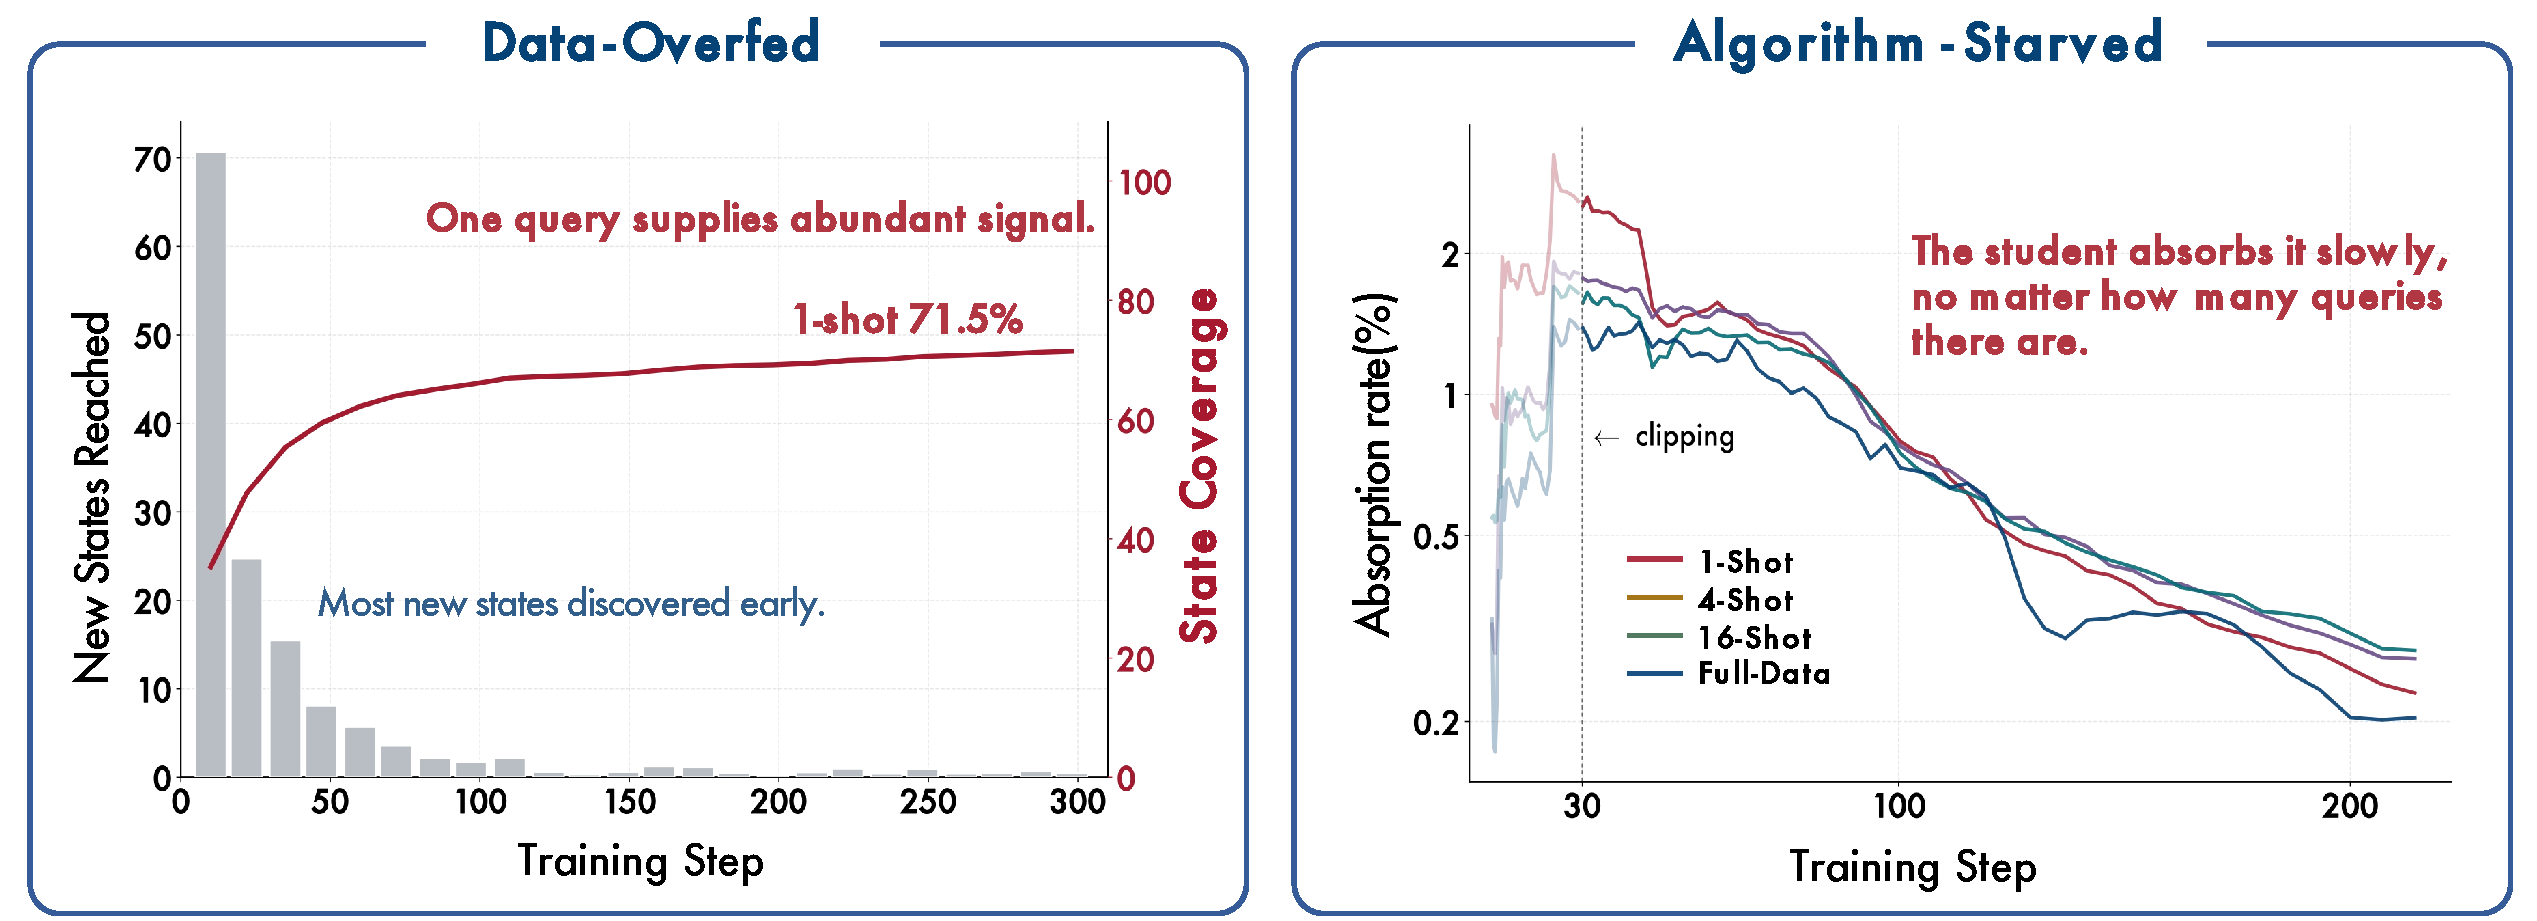
\includegraphics[width=\linewidth]{figures/main2.pdf}
    \caption{\textbf{OPD存在数据过载但算法匮乏的问题。} \textbf{数据：} 一次查询已覆盖大部分全数据OPD访问的状态。 \textbf{算法：} 无论学生模型训练了多少次查询，其吸收剩余教师-学生差距的比例始终越来越小。}
    \label{fig:overview}
\end{figure}

这个问题揭示了同策略教学（OPD）效率的两个方面，而标准训练将它们纠缠在一起：
\textit{\textbf{持续学习如此之久}} 关注的是 \textit{算法} 吸收监督信号的速度，而 \textit{\textbf{提升如此之大}} 则关注为何少量的 \textit{数据} 便足以提供充分的监督。
通过将数据供给缩减至极小点，one-shot OPD 将这两个方面解耦，而这一现象本身表现出很强的鲁棒性：其增益在四个任务领域和三个模型家族中均成立，并且即使在学生从未解决过的查询上依然有效 (\Cref{sec:one-shot})。
我们的答案是：\textbf{OPD 是数据过饱但算法饥饿}。
从 \textit{数据视角} 看，一个查询通过其轨迹所达到的 \emph{状态} 作用于学生，每个状态都是一个前缀 \(s=(x,y_{<i})\) ，在此处教师提供 token 级别的监督，因此一个查询集的价值取决于其所覆盖的状态空间部分。我们通过 \emph{状态覆盖} 来量化这一点：我们将全数据 OPD 所访问的状态分组为语义簇，并报告某一情景下轨迹所达到的比例。单个查询本身已能提供足够的状态，覆盖全数据 OPD 所访问内容的 \(71.5\%\) ，而 16 个语义多样性的查询则覆盖了 \(98.9\%\) 并达到了全数据训练的效果 (\Cref{sec:data})。这就是为何如此少的数据却能极大提升学生表现的原因。从 \textit{算法视角} 看，随着训练进行而下降的是 \emph{吸收率}，即一次更新能够弥补的剩余师生差距比例，其下降趋势在单个查询与全部 17k 查询上几乎相同 (\Cref{sec:algorithm})，因此运行速度是 OPD 本身的特性，而非训练集的属性。
换句话说，单个查询所提供的监督在很大程度上未被充分利用，其利用速率受限于同策略学生吸收信息的速度。

相同的机制同样适用于超越 one-shot 情景的数据设计。在多教师 OPD（MOPD）~\citep{xiao2026mimo,xu2026deepseek} 中，单个学生在多个领域上进行训练，每个查询被路由到其对应领域的教师，我们发现每个领域只需 16 个语义多样性的查询即可达到全数据训练的效果 (\Cref{sec:mopd})。将数据设计推向极致，我们进一步表明，即使一个不描述任何问题的训练输入仍可保持有效性：跨领域 WildChat 提示和无内容模板对 OPD 的驱动效果几乎与完整训练集相当 (\Cref{sec:template})。因此，输入之所以有效，主要在于它能够启动学生的推理过程。此外，我们在相同查询上对 one-shot RLVR 进行了受控对比，以明确算法差异：在几乎每次滚动中，一旦查询被解决，RLVR 的奖励即被耗尽；而 OPD 的 token 级信号在整个训练过程中持续存在，且 OPD 在 $1000$ 步内的验证增益超过 RLVR 的两倍 (\Cref{sec:opd-vs-rlvr})。

简而言之，OPD 所获得的监督信息超出了其算法所能吸收的范围。因此，数据监管需要解决的问题不再是收集多少问题，而是输入所引发的状态是什么。我们希望这种对训练数据的状态层面的理解，能为未来通过所引发的状态来选择查询，以及提高学生吸收这些信息的速率提供指导。
